\Introduction
\label{chap:introduction}

L'informatique graphique, branche du domaine de l'informatique, est l'étude de la création d'images numériques par ordinateur~\cite{poinssac_infographie_1994}. C'est un domaine à l'intersection de plusieurs disciplines, comme l'informatique, les mathématiques, la physique, l'optique, la biologie, et d'autres encore. L'informatique graphique trouve ses applications dans de nombreux autres domaines~\cite{ekaran_when_2021}, notamment celui du divertissement. Un défi de l'informatique graphique qui se dresse depuis ses débuts est celui de la création de contenu, car c'est un processus long et coûteux. Dans la figure~\ref{fig:hades} par exemple, le personnage, les bâtiments et leur architecture, la rivière et les effets de lumières sont tous des éléments qui ont dû être créés par une équipe d'artistes. Il existe diverses méthodes pour créer du contenu~\cite{juegoadmin_why_2023} dont plusieurs, comme le modelage 3D, qui demandent beaucoup de temps de travail aux artistes. De nos jours en particulier, il y a une demande croissante pour des univers virtuels de plus en plus grands et détaillés~\cite{imam_open_2022}. Les méthodes de création de contenu traditionnelles, par le pur travail manuel des artistes, sont de moins en moins viables en raison de la quantité de contenu nécessaire à créer pour remplir ces univers~\cite{freiknecht_survey_2017}. Il est nécessaire de mettre au point des méthodes plus automatisées pour permettre une création plus rapide et moins coûteuse.

\bigskip

\begin{figure}[!h]
    \centering
    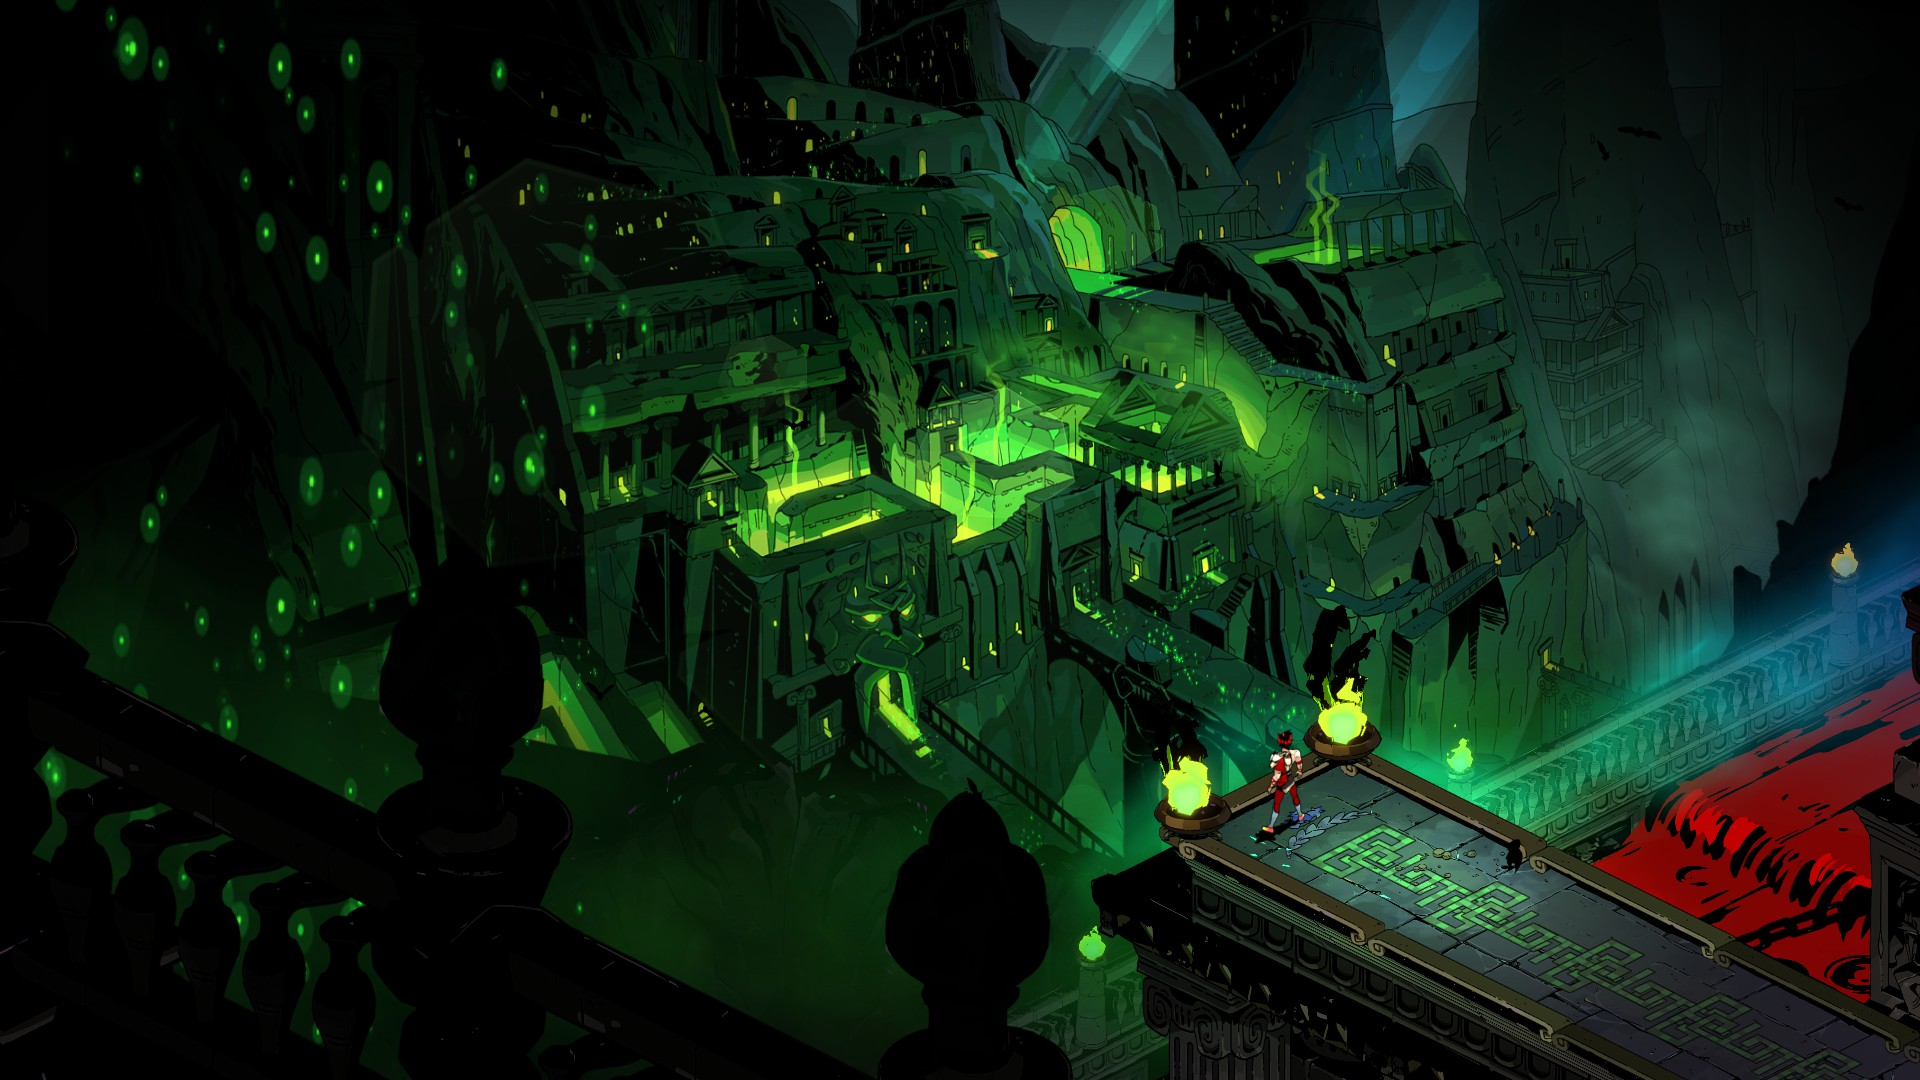
\includegraphics[width=.85\textwidth]{contenu/resources/images/hades}
    \caption{{\it Hades} (2018), Supergiant Games}
    \label{fig:hades}
\end{figure}

Dans ce contexte de méthodes automatisées, la génération procédurale est un procédé utilisé pour produire toutes sortes de ressources numériques~\cite{smelik_survey_2014}. La génération procédurale est en particulier utilisée pour synthétiser l'apparence visuelle des différents composants des scènes virtuelles~\cite{alessio_procedural_2021}. En combinant des méthodes algorithmiques avec de l'aléatoire, il est possible de générer des cartes de texture qui servent à habiller les mondes virtuels. Une carte de texture désigne une image qui est appliquée sur une surface pour lui donner un aspect visuel dans le but d'accentuer l'immersion des utilisateurs. Différentes textures nécessitent différentes méthodes de synthèse pour être générées. Certains genres de textures sont encore difficilement réalisables avec les méthodes existantes~\cite{lutz_cyclostationary-gaussian_2021}. C'est dans cette perspective que s'inscrit ce travail de recherche, qui a pour but d'approfondir notre compréhension des éléments qui constituent la structure d'une image. Ce travail explore l'analyse multi-résolutionnelle locale et son application à la synthèse de texture procédurale. L'analyse multi-résolutionnelle locale est un outil du domaine du traitement du signal et est détaillée dans la suite de ce manuscrit~\ref{chap:chapitre1}.

\section{Monde virtuel}

Dans le cadre de l'informatique graphique, un monde virtuel est une méthode de représentation de scènes au moyen d'un support numérique. Une scène est une collection d'objets numériques qui interagissent entre eux. Il existe trois sortes d'objets numériques qui composent une scène : de la géométrie, des lumières et des caméras. Avec des algorithmes dits de \og rendu \fg, un monde virtuel peut être converti en image. Les mondes virtuels sont utilisés dans de nombreux domaines~\cite{magnenat-thalmann_introduction_1986}, comme :

\begin{itemize}
    \item le domaine du divertissement, pour les jeux vidéo (l'industrie du jeu-vidéo est un des principaux acteurs des avancées en graphisme) ;
    \item le domaine de l'animation, pour les films d'animation ou les effets spéciaux de films ;
    \item le domaine médical, pour des outils de visualisation de l'anatomie humaine ou de formation en réalité virtuelle ;
    \item le domaine de l'ingénierie, pour aider à la conception d'objets (Conception Assistée par Ordinateur) ou de bâtiments (architecture) ;
    \item le domaine militaire, pour faire des simulations de situations ou des entraînements au combat.
\end{itemize}

\subsection*{Types de rendu}

La visualisation de scènes virtuelles s'opérationnalise au travers d'un logiciel dit \og moteur de rendu \fg utilisant divers algorithmes pour fonctionner~\cite{sherman_chapter_2003}. Un moteur de rendu traite une scène en différentes étapes dans le but de créer une visualisation de cette scène, appelée \og rendu de la scène \fg. Il existe plusieurs méthodes de rendu qui implémentent différents algorithmes pour produire différentes visualisations d'une scène. Pour exécuter leurs calculs, les logiciels de rendu s'appuient sur les capacités des cartes graphiques ({\it Graphics Processing Unit} ou GPU). Les GPUs sont des processeurs hautement parallèles et spécialisés dès leur fabrication pour des calculs graphiques~\cite{das_history_2016}.

\bigskip

\begin{figure}[h]
    \centering
    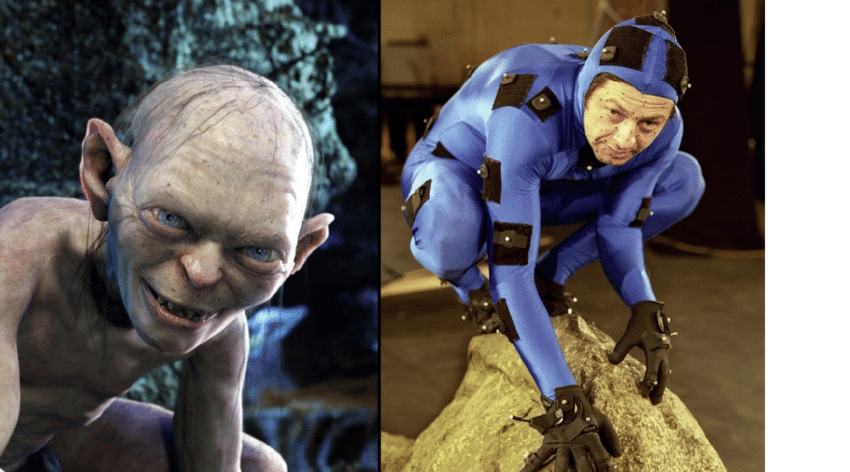
\includegraphics[width=.65\textwidth]{contenu/resources/images/gollum}
    \caption[{\it Gollum} (2002), {\it Le Seigneur des Anneaux : Les Deux Tours}]{{\it Gollum}, personnage complètement généré par image de synthèse par rendu hors-ligne. {\it Le Seigneur des Anneaux : Les Deux Tours}, Peter Jackson~\cite{jackson_lord_2002}. Image par Mou~\cite{mou_keyframe_2018}.}
    \label{fig:gollum}
\end{figure}

Les méthodes de rendu peuvent être séparés en deux grandes catégories : le rendu \og hors-ligne \fg et le rendu \og en temps-réel \fg. Le rendu hors-ligne désigne les algorithmes qui font la visualisation de scènes non interactives, où il n'est pas possible de contrôler les interactions entre les éléments de la scène. Les films d'animation ou les effets spéciaux de films~\ref{fig:gollum} sont des exemples de rendus fait hors-ligne. L'utilisation de méthodes de rendu hors-ligne est en fait devenu une norme dans l'industrie cinématographique~\cite{media_history_2021}, car elle permet la création de scènes qu'il serait impossible de tourner à l'aide de caméras traditionnelles. À l'inverse, lors d'un rendu en temps-réel, une personne utilisatrice a un contrôle sur la scène qui est rendue pendant qu'elle est rendue. Le déplacement d'un personnage dans un jeu-vidéo, la manipulation d'un modèle de pont dans un logiciel d'architecture et l'affichage d'objets dans une application de réalité augmentée sont tous des exemples de rendus en temps-réel. Une même scène peut être rendue avec plusieurs méthodes de rendu, la visualisation finale sera alors différente à chaque fois. Une scène rendue en temps-réel d'une part et hors-ligne d'autre part, est montrée à la figure~\ref{fig:zero-day}. Les enjeux et contextes des rendus hors-ligne et en temps-réel diffèrent. Le travail présenté dans ce manuscrit s'intéresse aux méthodes de rendu en temps-réel. Dans la méthode proposée, bien qu'une partie de préparation des données soit nécessaire, le rendu final se fait en temps-réel. Les problématiques et solutions concernant le rendu hors-ligne ne sont donc pas abordées dans ce travail.

\bigskip

\begin{figure}[h]
    \centering
    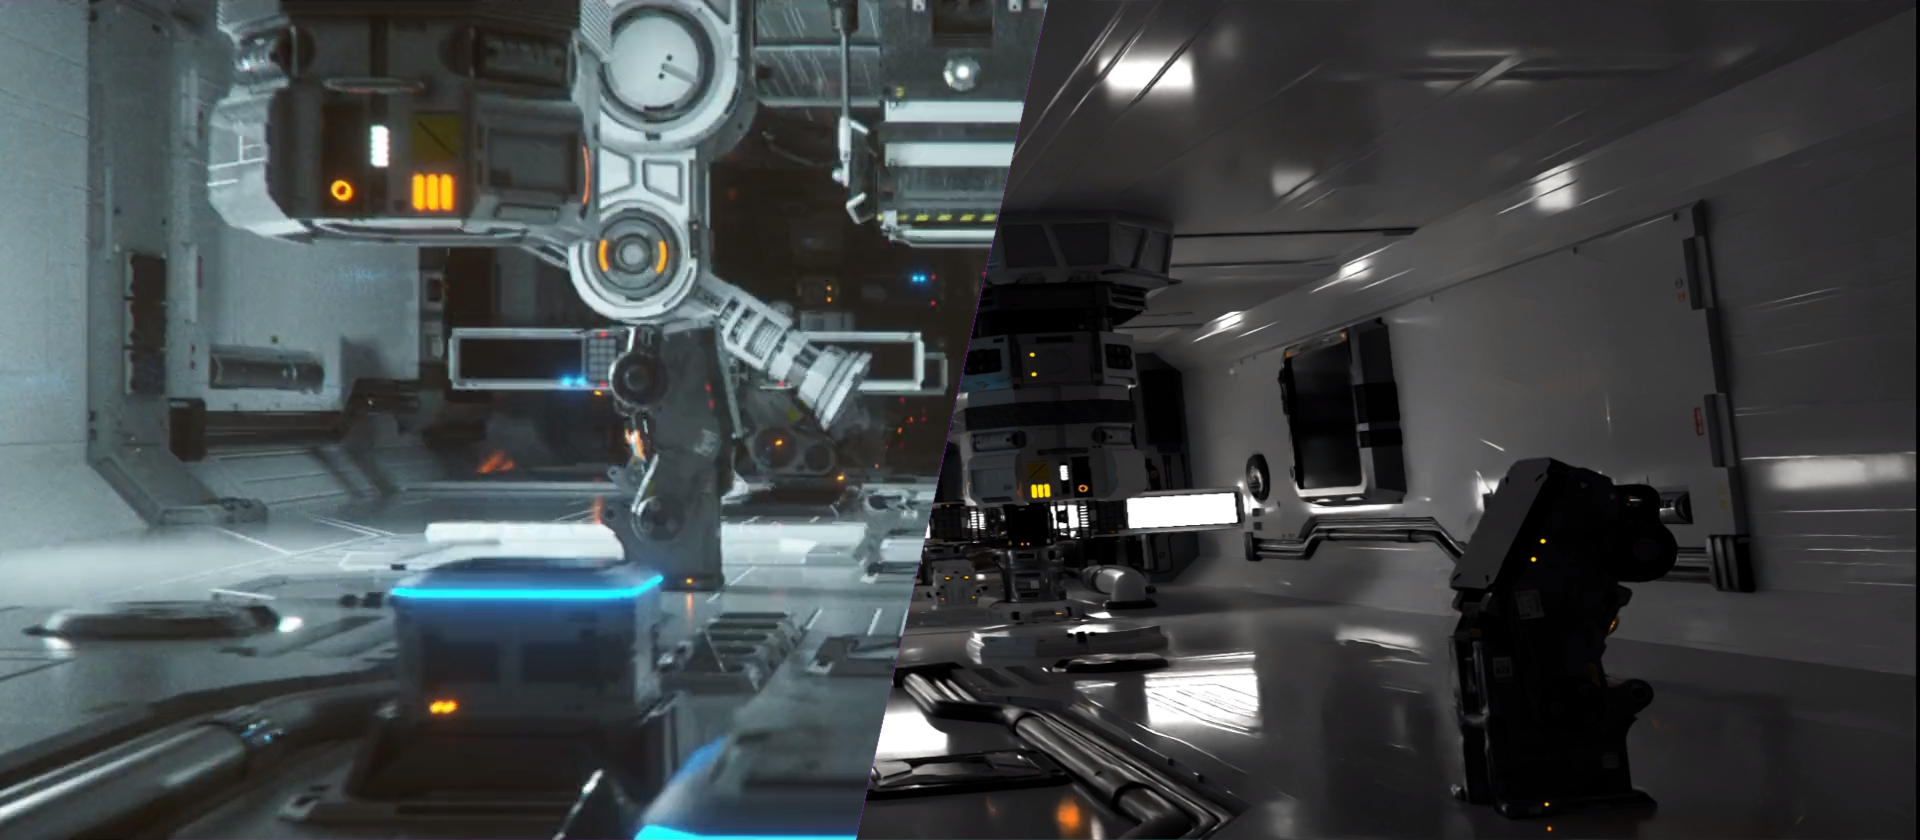
\includegraphics[width=\textwidth]{contenu/resources/images/zero_day_comparison}
    \caption[{\it Zero-Day} (2015), BEEPLE]{{\it Zero-Day} (2015), BEEPLE. À gauche rendu original hors-ligne, à droite rendu temps-réel par SY tracé de chemins, NVIDIA~\cite{ZeroDay}}
    \label{fig:zero-day}
\end{figure}

Une méthode de rendu en temps-réel doit répondre à certaines contraintes dues à la nature interactive de la scène. Le rendu de la scène ne peut pas se faire en avance, car la scène est modifiée pendant l'utilisation. Le rendu doit être assez rapide pour afficher les images assez vite de telle sorte que le flux soit continu à l'œil humain. L'industrie cinématographique utilise un standard de 24 images par secondes pour l'enregistrement de films~\cite{deguzman_why_2023}. Pour un rendu en temps-réel, les applications visent des objectifs d'au moins 30 ou 60 images par secondes, afin que le contrôle utilisateur soit confortable~\cite{janzen_is_2014}. Les algorithmes utilisés doivent ainsi être conçus pour s'exécuter avec moins de temps, moins de ressources de calcul, et moins d'espace mémoire disponible.

\subsection*{Maillage}

% TODO intro avec source de ce qu'est un maillage
% TODO terme de représentation à définir un peu plus, qu'est ce qu'une représe
% source source source

Idéalement, on aimerait représenter les objets des scènes virtuelles de manière continue et exacte, mais une telle représentation est difficilement accessible. Comme solution pratique, on choisit d'utiliser des \og maillages \fg, des grilles de polygones (souvent des triangles) qui sont une approximation de notre géométrie, approximation dont la complexité et la densité peuvent varier selon les besoins. Les maillages étant stockés comme des tableaux de points et de faces, il se pose en effet des questions de coût en espace mémoire et de temps d'exécution des calculs qui sont effectués sur ces maillages par la suite, surtout dans le cas du rendu temps réel.
% TODO réécrire en style scientifique (voir propal nico)
% question du cout memoire + temps execution p-e pas nécessaire vu que non utile dans travail

\begin{figure}[h!]
    \centering
    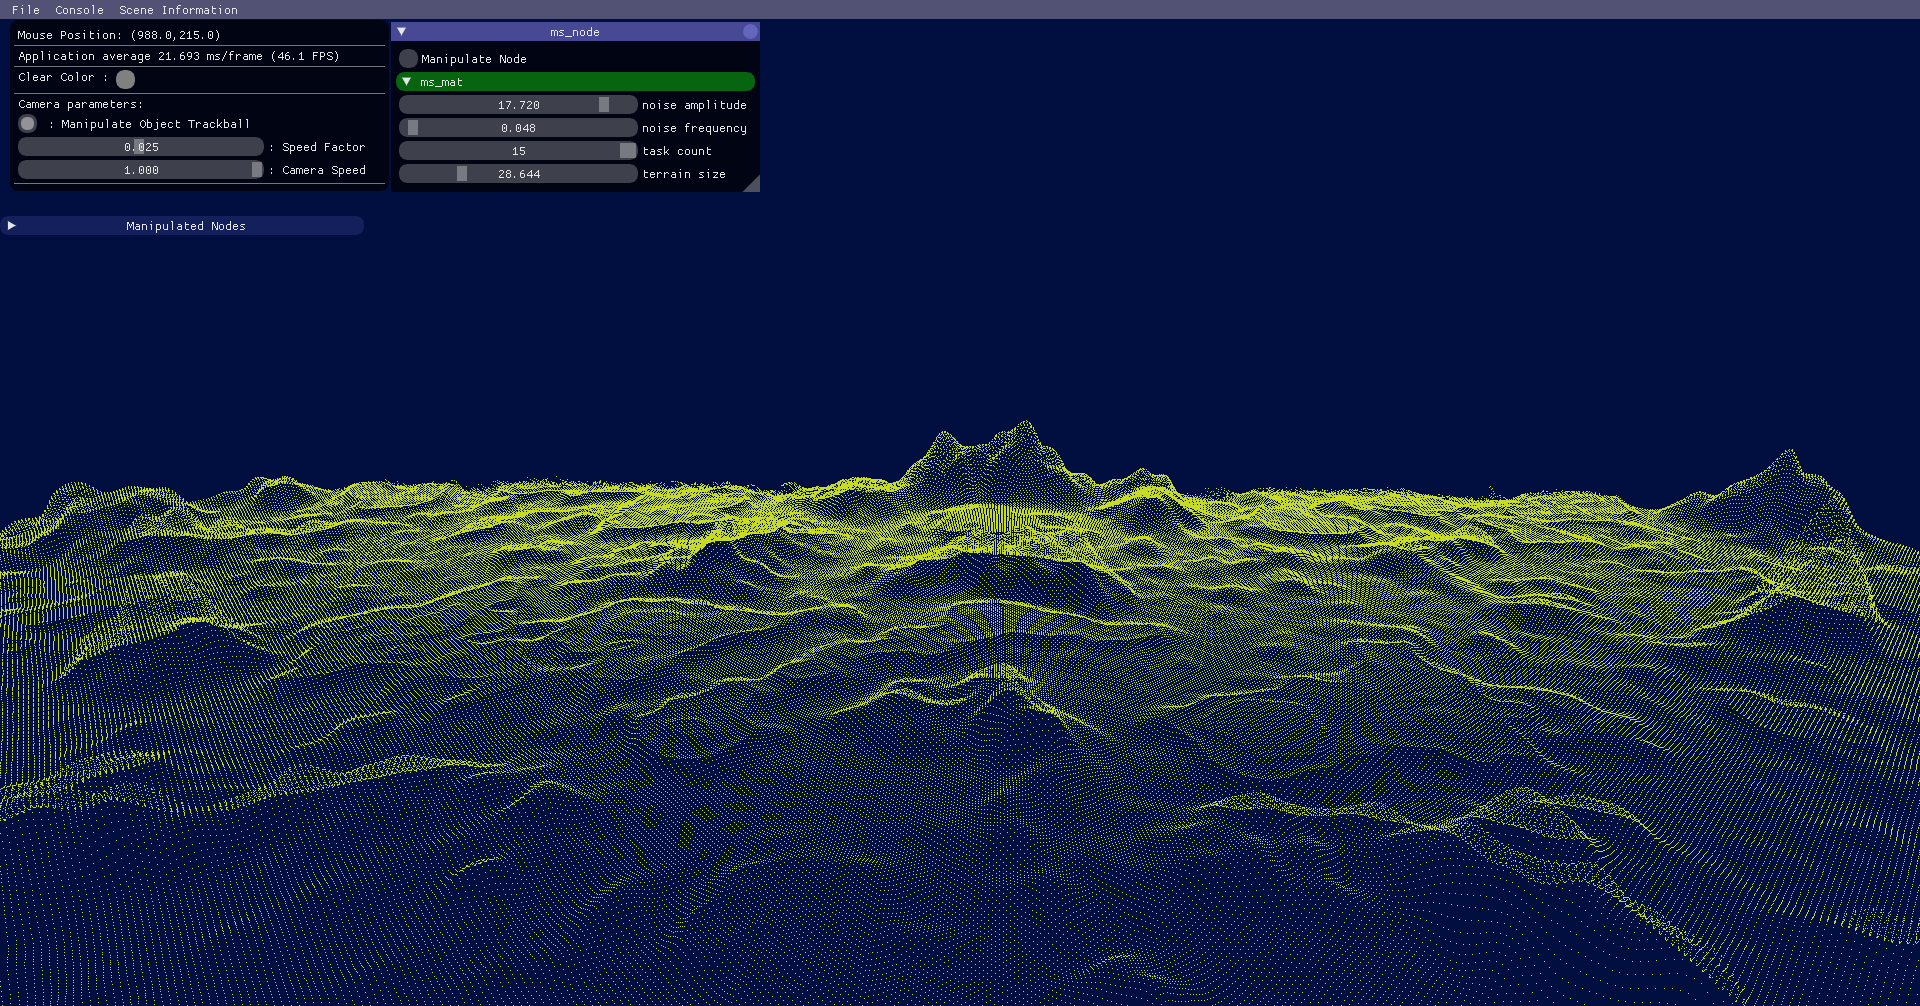
\includegraphics[width=\textwidth]{contenu/resources/images/full_terrain}
    \caption{Maillage d'un terrain généré procéduralement}
    \label{fig:procedural-mesh}
\end{figure}

\section{Texture}

\subsection*{Plaquage de texture}

%TODO positionnement par rapport aux micro mesh ?
% TODO "trop" de details -> eclaircir
Le maillage seul ne suffit cependant pas à représenter parfaitement la géométrie, qui a trop de détails pour la résolution des maillages RE tractables avec la technologie actuelle. Pour remédier à ce problème, on utilise des \og textures \fg, qui ajoutent les détails manquants à une géométrie simplifiée. De manière générale, on appelle texture une fonction d'un espace de coordonnées, habituellement deux ou trois dimensions, vers un espace de valeurs numériques à une ou plusieurs dimensions. Les dimensions de l'espace d'arrivée sont appelées \og canaux \fg de la texture. Ils représentent généralement une couleur (RGB ou RGBA), mais peuvent aussi correspondre à d'autres grandeurs (scalaires par exemple) qui encodent des valeurs physiques utiles au rendu de la scène, comme une profondeur, une hauteur ou un vecteur normal par exemple. La majorité du temps, les textures sont stockées en mémoire comme des images, des tableaux multi-dimensionnels finis de données, que l'on appelle alors des \og cartes \fg.
%TODO opposer ici discret vs continu procédural
% TODO conseil nico pour mieux reformuler
% TODO source pour la méthode de plaquage de texture ?

\bigskip

Pour une même surface, il est courant d'utiliser plusieurs textures pour calculer l'éclairage et la couleur. Les textures en question dépendent du modèle d'éclairage utilisé. Le format de rendu physique réaliste ({\it Physically Based Rendering} ou PBR), standard de l'industrie, nécessite typiquement cinq cartes de texture : l'albedo (ou couleur), mais aussi la normale, la hauteur, la rugosité et l'occlusion ambiante.
% source pbr standard industrie

\bigskip

\begin{figure}
    \centering
    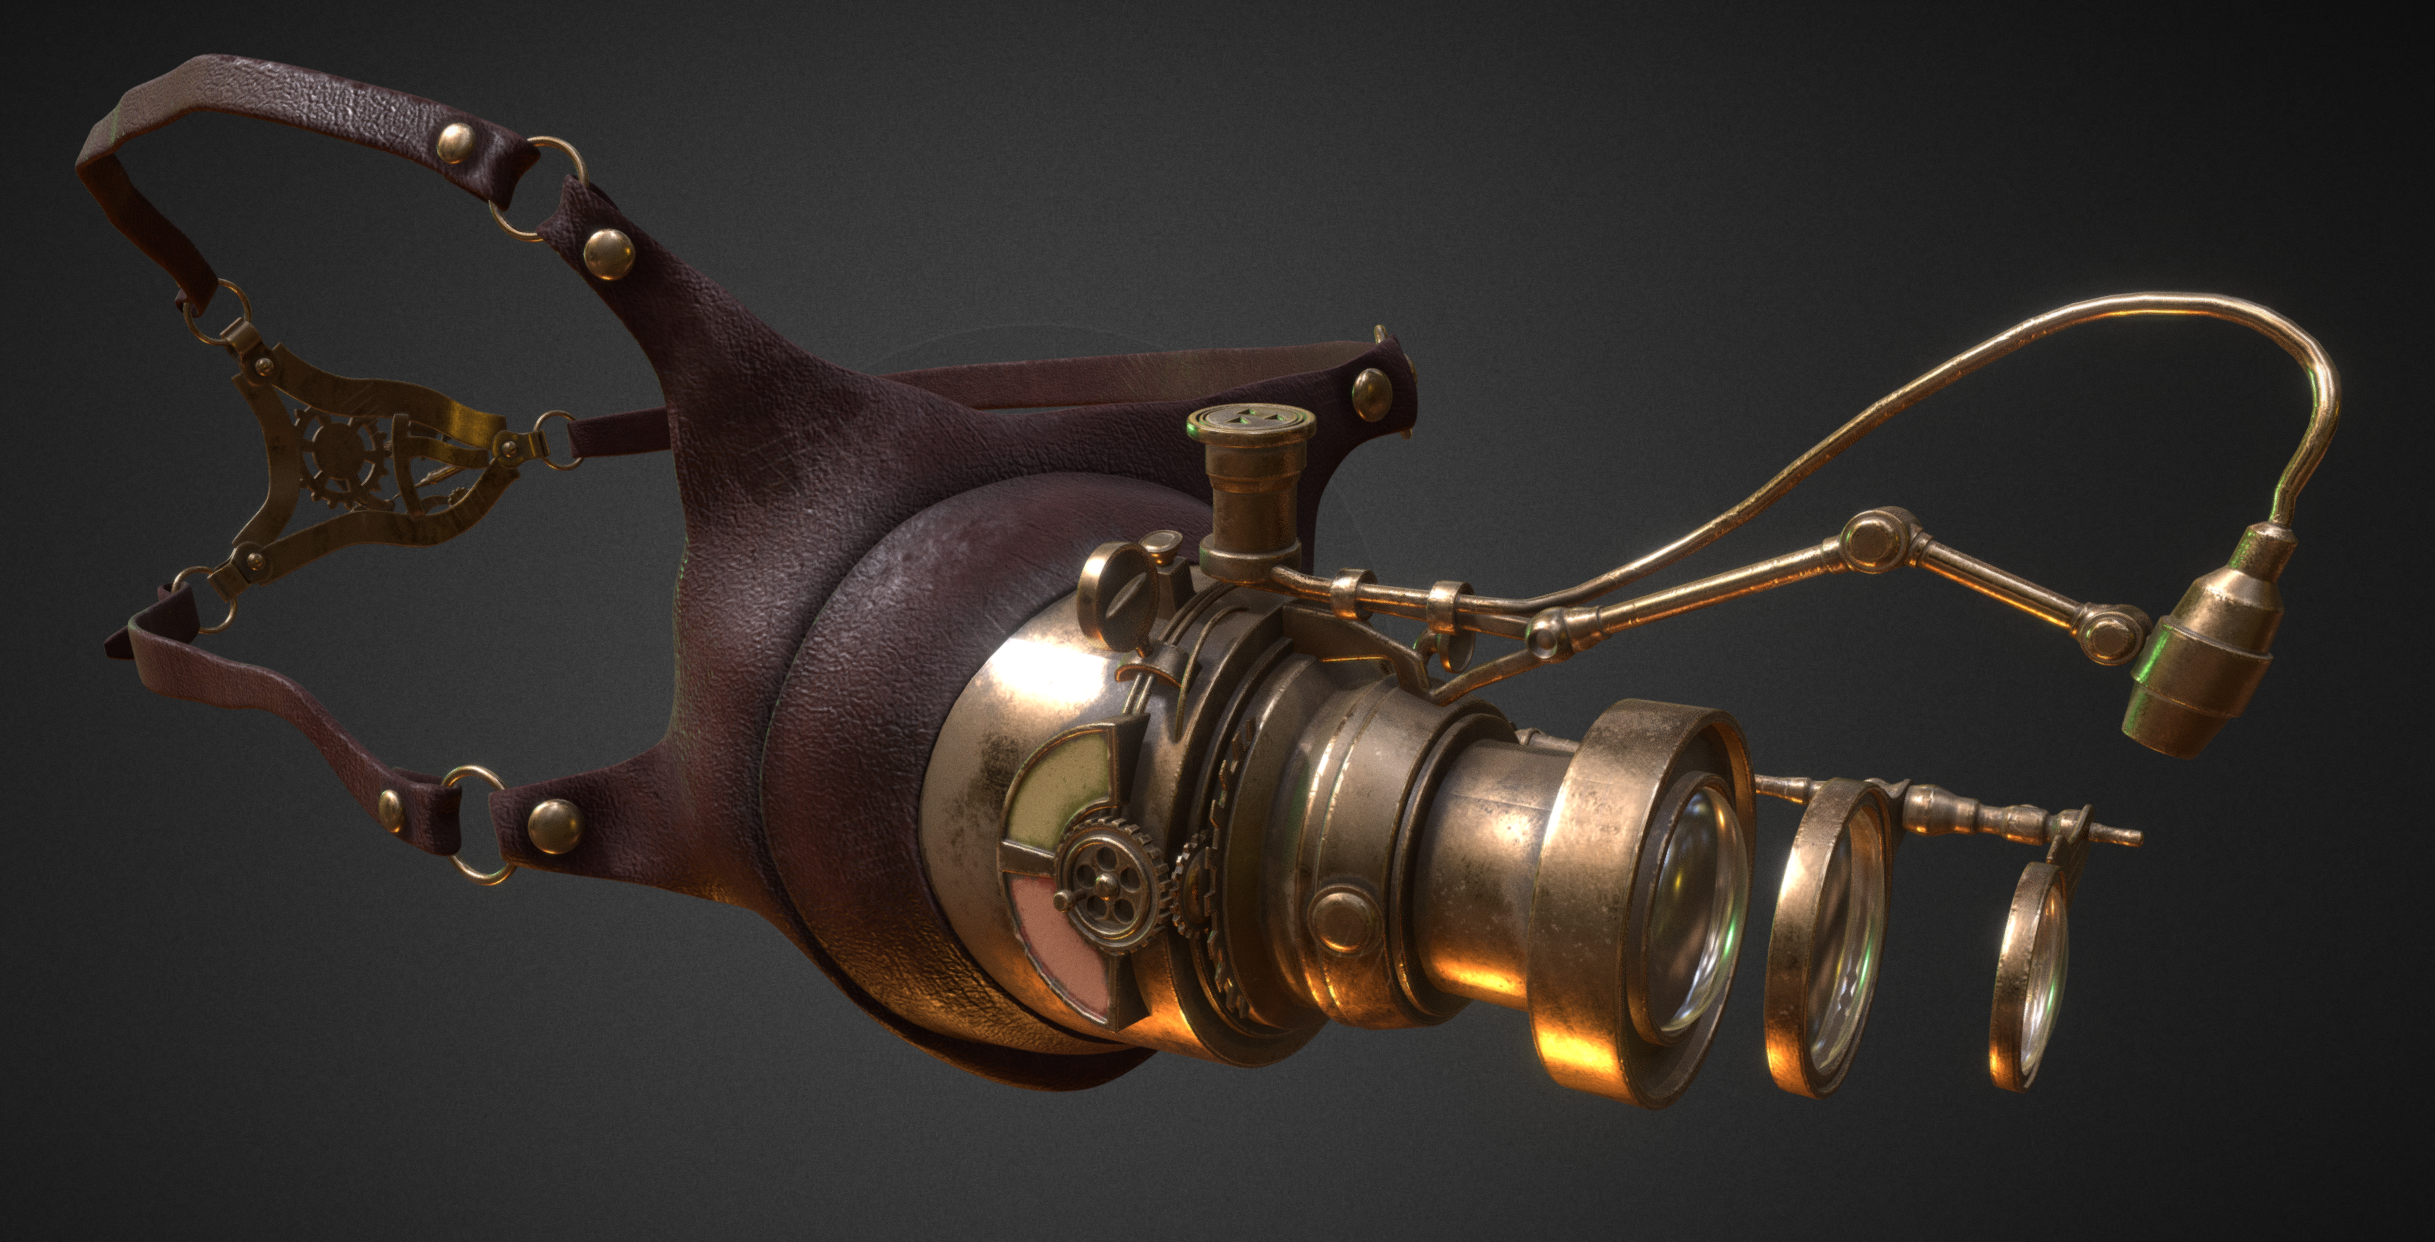
\includegraphics[width=.65\textwidth]{contenu/resources/images/mutli-material-object}
    \caption[Rendu d'un objet comportant plusieurs matériaux]{Plusieurs matériaux différents sont utilisés pour le rendu de cet objet~\cite{multi-material}}
    \label{fig:multi-material}
\end{figure}

La méthode de travail usuelle en industrie consiste à regrouper ces différentes textures, ainsi que le modèle d'éclairage, dans un \og matériau \fg. Les objets d'une scène sont ainsi composés de plusieurs matériaux, qui présentent chacun des propriétés physiques différentes. Une chaise peut par exemple avoir une armature en bois, un recouvrement en cuir et des clous en métal. Pour créer leurs scènes, les artistes façonnent ainsi leurs objets en commençant par la géométrie, avant de créer (ou réutiliser) les différents matériaux pour habiller leurs objets.
% todo source source source

\subsection*{Échantillonnage}

% TODO première phrase p-e cheloue voir nico
L'intérêt de la texture est donc d'augmenter la quantité de détails de notre rendu à faible coût, puisque la géométrie sous-jacente reste plus grossière, et que la résolution de cette dernière est un des facteurs majeurs de ralentissement du rendu d'une scène. Pour plaquer des textures, qui souvent sont des images carrées, sur une surface quelconque, on utilise un système de coordonnées, dites UV, qui permet d'aligner les deux comme souhaité. Les coordonnées UV, un vecteur entre $(0, 0)$ et $(1, 1)$, sont définies pour tous les sommets au moment de la création du maillage. On peut alors utiliser ces coordonnées comme argument de la texture, dont l'espace de coordonnées de départ est aussi entre 0 et 1.
% TODO : "aligner les deux comme souhaité" = immprécis

\bigskip

\begin{figure}
    \centering
    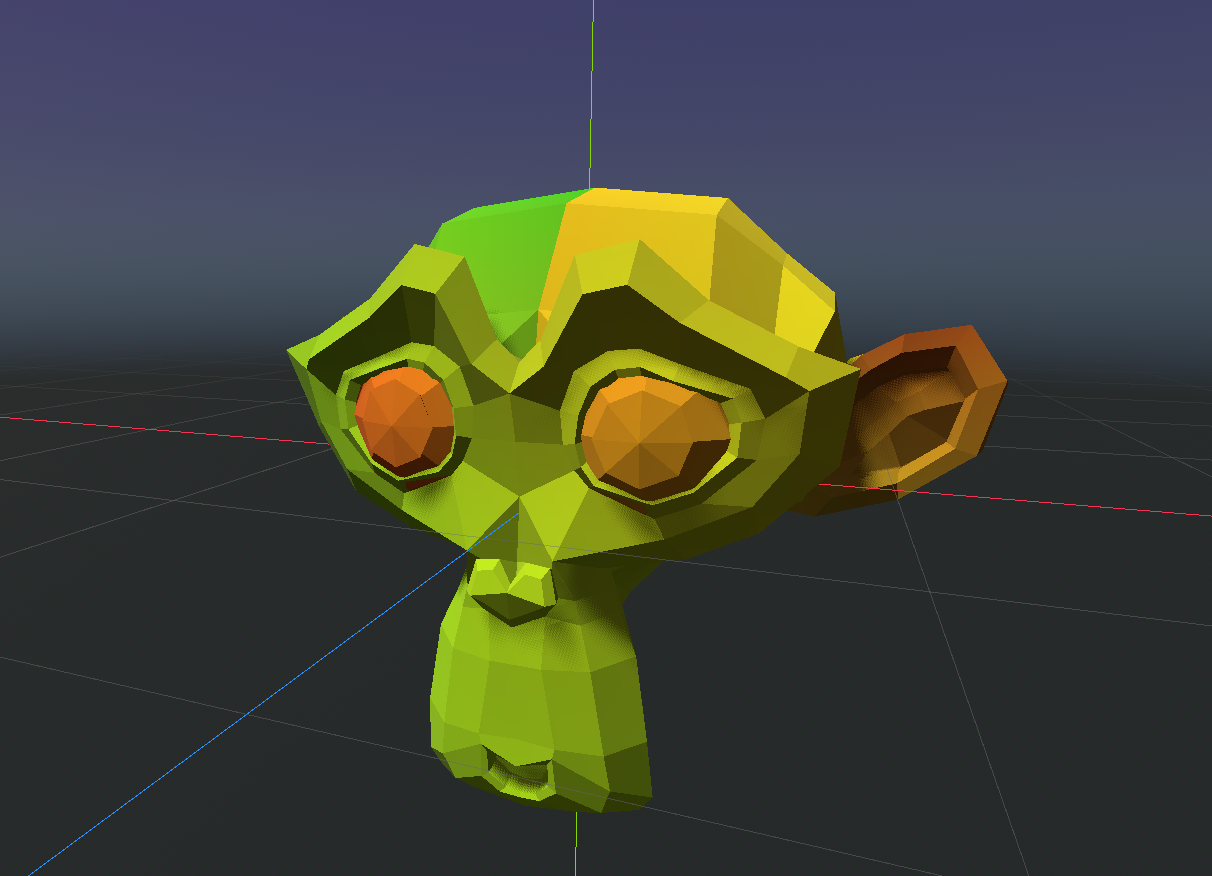
\includegraphics[width=.55\textwidth]{contenu/resources/images/uv_suzanne}
    \caption[Coordonnées UV du modèle Suzanne]{Visualisation des coordonnées UV de Suzanne~\cite{suzanne-uv}, modèle 3D de référence du logiciel Blender}
    \label{fig:uv-suzanne}
\end{figure}

Cette étape dite d' \og échantillonnage \fg s'effectue au moment du rendu. Dans le \textit{pipeline graphique} de rastérisation, utilisé classiquement pour faire du rendu interactif, la scène est projetée sur le plan image, puis découpée en \og fragments \fg de taille inférieure aux polygones formant le maillage des objets de la scène. Les fragments ont une valeur de coordonnée de texture, souvent notée \og coordonnée UV \fg, interpolée entre les valeurs des sommets voisins et peut donc aller interroger les textures pour récupérer les valeurs aux bons endroits.
% TODO paragraphe/explication à retravailler, confusant
% TODO voir nico pour aide reformulation
% Faire le lien entre fragments et pixels

\subsection*{Filtrage}
%TODO pertinence de la section ? ext ce que j'utilise ça dans mon travail ?

La rastérisation pose cependant des problèmes dûs à l'encodage discret des textures en image. Les fragments rastérisés et les texels de texture échantillonnés représentent tous les deux des surfaces de petite taille, caractérisés par des coordonnées uniques. Il se peut néanmoins que les surfaces couvertes par les deux ne soient pas les mêmes, même si les coordonnées UV sont identiques ; c'est particulièrement le cas lorsque la taille du fragment et celle du texel sont différentes.
% TODO revoir le paragraphe (voir annotations guillaume)
% TODO voir nico pour reformulation et lien entre P et e(P)
% utiliser et citer la figure, souligner la correspondance P et e(P)
% TODO def texel

\bigskip

\begin{figure}
    \centering
    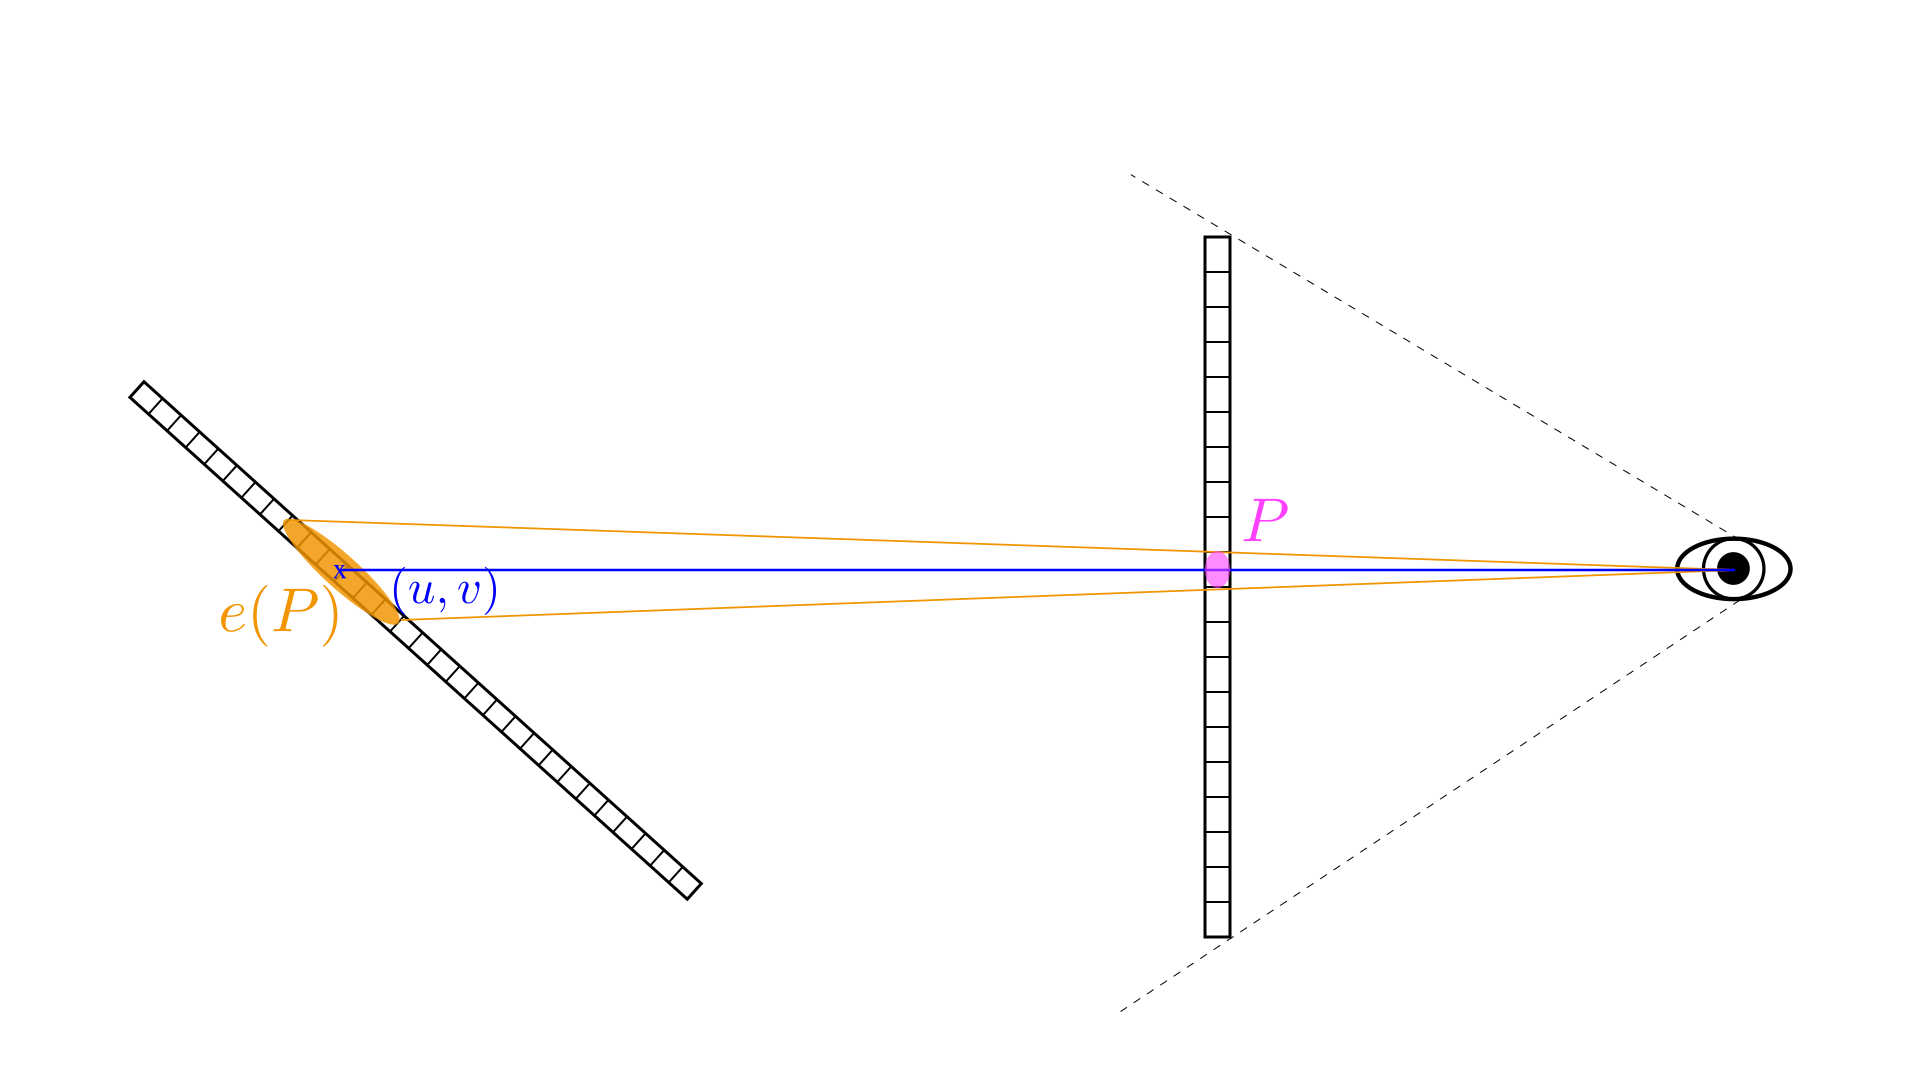
\includegraphics[width=\textwidth]{contenu/resources/images/schema_filtrage}
    \caption[Visualisation du problème d'échantillonnage lors du rendu par rastérisation]{À cette distance de l'écran, l'empreinte du fragment $e(P)$ couvre plusieurs texels. Les coordonnées $(u, v)$ ne sont pas suffisantes pour capturer toute l'information.}
    \label{fig:aliasing}
\end{figure}

Il faut alors employer des méthodes dites de \og filtrage \fg pour corriger l'échantillonnage, car la différence de taille entre les fragments et les texels cause des artefacts visuels appelés \og aliassage \fg. Pour des textures standards, il existe différentes méthodes de filtrages utilisées couramment :
% TODO def artefacts visuels

\begin{itemize}
    \item \textbf{Sur-échantillonnage} : lorsque le fragment est plus petit que le texel, plusieurs fragments voisins peuvent prendre la même valeur. Cela donne un aspect crénelé, avec les contours des objets en escalier. La solution idéale dans ce cas serait d'augmenter la résolution de la texture utilisée ; ce n'est cependant pas tout le temps possible. Comme alternative, au lieu d'attribuer au fragment la valeur du texel correspondant, on interpole la valeur des quatre texels voisins. On réduit l'aspect pixélisé, au prix d'un échantillonnage plus coûteux et d'un effet de flou sur l'image.
    \item \textbf{Sous-échantillonnage} : lorsqu'un fragment est plus grand qu'un texel~\ref{fig:aliasing}, et qu'il en recouvre plusieurs, alors plusieurs fragments voisins peuvent être très espacés sur la texture et on perd l'information des texels entre. De loin, on aperçoit un motif de moiré et l'image scintille lorsque l'on change légèrement l'angle de vue. La solution idéale serait ainsi de prendre en compte tous les texels touchés et faire une intégrale de la valeur de la texture sur toute la surface couverte par le fragment, ce qui est très souvent irréalisable. L'alternative classique consiste à pré-calculer différentes échelles de la texture utilisée, appelées \og MIP maps \fg, et de trouver l'échelle adéquate de telle sorte qu'un texel ait la même taille qu'un fragment. L'échantillonnage est plus lourd et on prend plus d'espace mémoire pour stocker les MIP maps, mais la texture est mieux rendue de loin.
\end{itemize}
% TODO paragraphe à revoir (voir annotations guillaume)
% TODO voir nico faire attention entre taille frag<->texel, parler d'empreinte
% TODO "échantillonnage plus lourd" whack, voir nico reformulation
% TODO source méthode de filtrage

\begin{figure}
    \centering
    \begin{subfigure}[b]{.45\textwidth}
        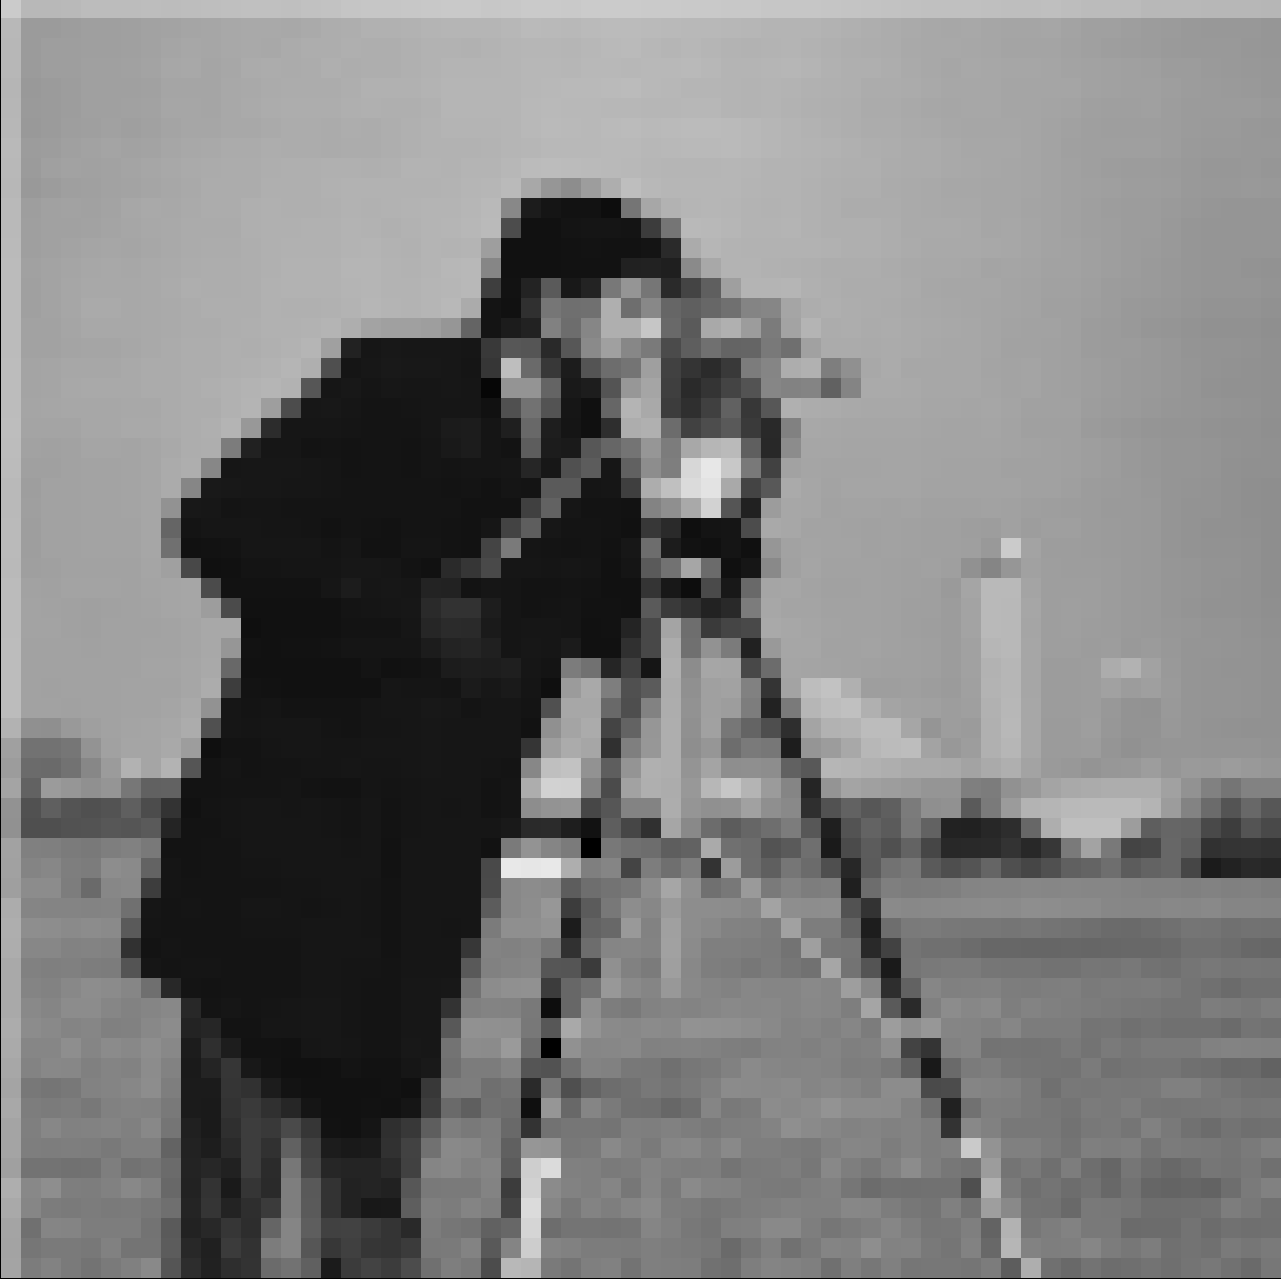
\includegraphics[width=\textwidth]{contenu/resources/images/cameraman_nearest}
        \caption{Sans filtrage}
    \end{subfigure}
    \hfill
    \begin{subfigure}[b]{.45\textwidth}
        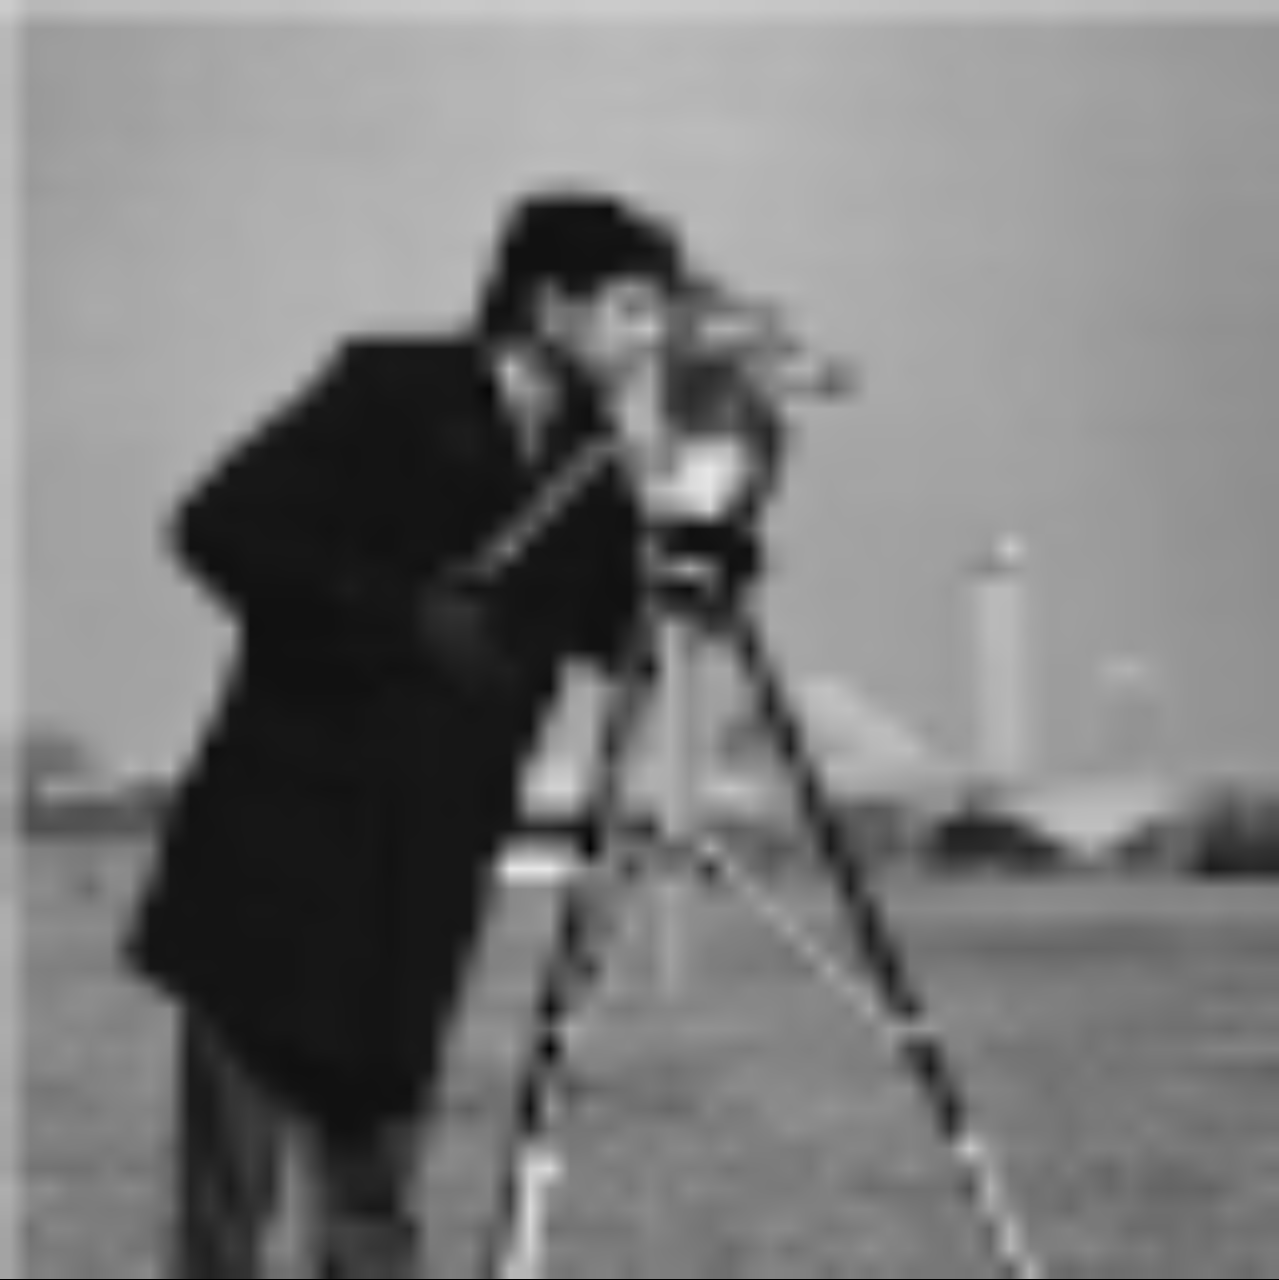
\includegraphics[width=\textwidth]{contenu/resources/images/cameraman_linear}
         \caption{Avec filtrage linéaire}
     \end{subfigure}
    \caption{Filtrer correctement est un enjeu majeur dans l'utilisation des textures}
    \label{fig:filtrage}
\end{figure}
% TODO changer image pour texture plus voir nico comment bien faire la figure

{\color{red}Pertinence de ce paragraphe ?}
De nombreuses méthodes de filtrage plus élaborées sont employées pour obtenir des résultats de meilleure qualité, ou pour filtrer des textures plus compliquées. Par exemple quand les textures ne sont plus des images prédéterminées à l'avance, mais qu'elles sont générées au moment du rendu.
% TODO oui pertinent, mentionner les autres solutions "idéales" mais plus difficiles (voir not)

\section{Synthèse de texture}
%TODO "bien souvent" vague
Bien souvent, les surfaces que l'on souhaite couvrir sont de grande taille, par exemple des sols. Produire et stocker des textures de même taille que les surfaces n'est pas toujours envisageable, le coût en temps de création et en empreinte mémoire est trop élevé. Étirer les textures en utilisant les coordonnées UV est une solution, qui atteint cependant ses limites assez rapidement : on remarque qu'une texture de plus basse résolution est utilisée. En rendu interactif, on résout le problème en synthétisant directement une texture de taille adaptée à notre surface. On peut catégoriser les types de texture existants de plusieurs manières ; pour le présent manuscrit, nous les distinguerons selon le niveau d'organisation des éléments qui les compose~\ref{fig:échelle-structure}.
% TODO mieux faire le lien et introduire partie d'après (voir not)
% TODO "catégorisation plusieurs manières" -> quelles sont les autres
% todo source pour les méthodes usuelles

\subsection*{Algorithme de synthèse}

On appelle \og synthèse de texture \fg un procédé qui permet de produire une texture de taille arbitraire, pouvant prendre en argument des paramètres de différente nature. Par extension, on qualifie aussi de synthèse le résultat d'un algorithme de synthèse. Les avantages à utiliser un procédé de synthèse sont multiples. La texture générée est infinie, il est donc facile de l'appliquer à des surfaces de taille quelconque, avec la résolution désirée. De plus, il n'est pas nécessaire de stocker la texture d'avance en mémoire puisqu'on l'évalue au vol, on réduit ainsi l'empreinte mémoire.
%TODO "les avantages à utiliser..." : Une texture périodique a aussi une taille non bornée et tous les algorithmes de synthèse ne génèrent pas des textures de taille non bornée; c'est une propriété possible d'un algorithme de synthèse (et souhaitée ici)

% Enfin, on a un grand degré de contrôle sur l'apparence de nos objets, même au sein d'une scène intéractive.

\bigskip

\begin{figure}[H]
    \centering
    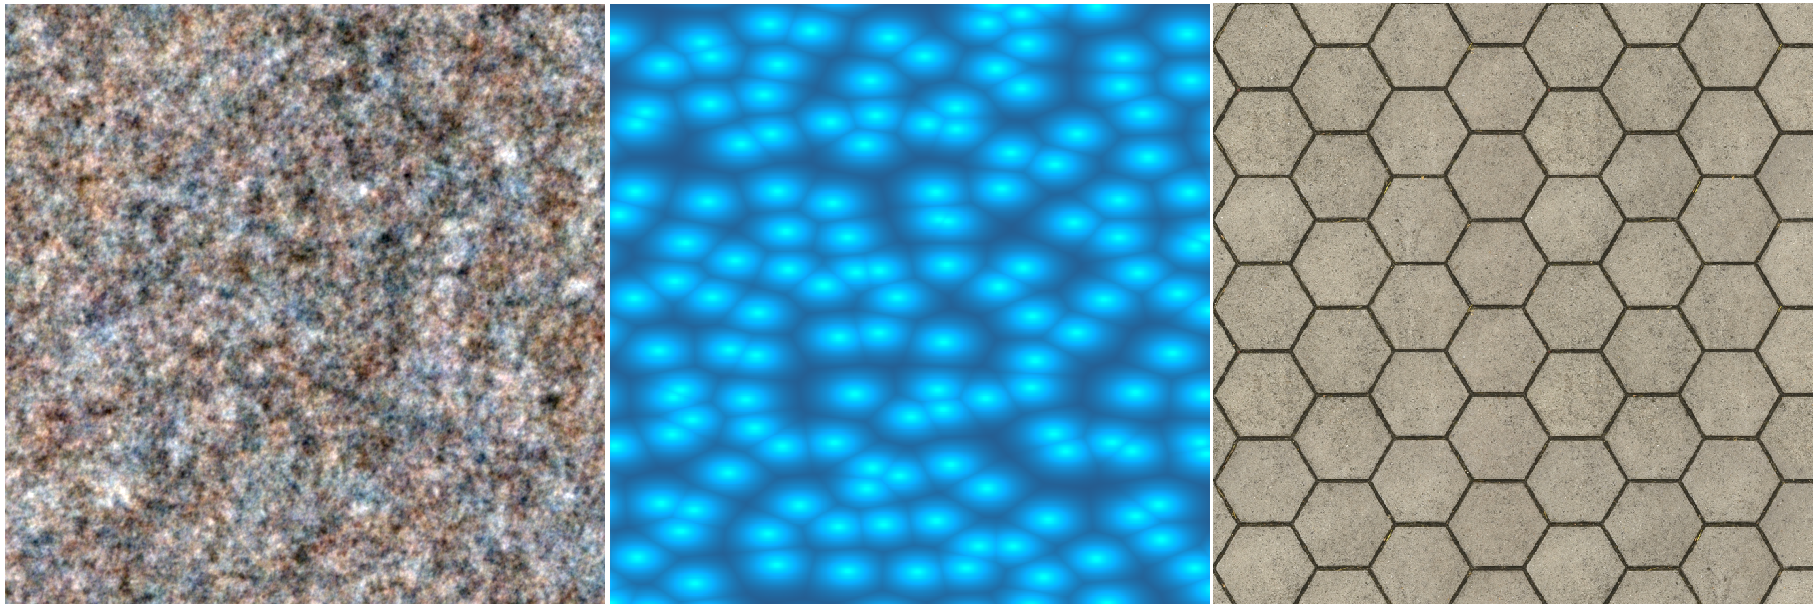
\includegraphics[width=\textwidth]{contenu/resources/images/structure_scale}
    \caption[Classification des textures selon leur niveau de structure]{Les textures peuvent être classées selon leur niveau de structure : stochastiques ou gaussiennes (gauche), semi-régulières (milieu), ou structurées (droite)}
    \label{fig:échelle-structure}
\end{figure}
% TODO changer image de droite, confusant avec périodicité

%TODO p-e parler de propriétés de synthèse, et présenter que les cas qui m'intéressent
Il existe plusieurs types de synthèses différentes, qui produisent des types de textures différentes. Une première distinction majeure que l'on peut faire est, comme pour le rendu, entre une synthèse hors-ligne et une synthèse en temps réel. Les ressources en temps et en puissance de calcul impliquées diffèrent, les enjeux ne sont souvent pas les mêmes. Nos travaux se focalisent sur le rendu et la synthèse temps-réel, on écarte de ce manuscrit les synthèses hors-ligne, comme les synthèses par optimisation ou par apprentissage profond (ou tout autre forme de réseau de neurones). Les algorithmes auxquels on s'intéresse ont comme contraintes de pouvoir s'exécuter pendant le rendu, sans que le budget de temps du rendu dépasse le seuil établi. Pour rentrer dans ces contraintes de temps, on exploite la puissance des GPUs, et notamment leur aspect hautement parallélisable. Les algorithmes de synthèse doivent donc pouvoir s'exécuter de manière parallèle, chaque texel doit pouvoir se calculer indépendamment des texels voisins ou à l'aide du voisinage proche uniquement.
{\color{red}PARLER DE la métrique des accès texture pour avoir une estimation de la vitesse ?}
% TODO selon G difficile ici
% TODO si je l'utilise pas dans mes travaux p-e pas (nico)
% Todo source pour dire que il erxiste  différents types de rendu

\subsection*{Synthèse temps-réel} % / Types de synthèse

Sous ces contraintes d'efficacité et de rapidité, de nombreux algorithmes subsistent ; deux grandes catégories de méthodes courantes sont la synthèse \og par réorganisation \fg et la synthèse \og par convolution \fg.

\subsubsection{Synthèse par réorganisation}

Le but d'une synthèse par réorganisation est de reproduire un extrait de texture donné en entrée en réutilisant et réagençant des morceaux dits « tuiles », de l'exemple. Plusieurs paramètres comme la taille, découpe, forme et disposition des tuiles peuvent être modifiés pour faire varier la synthèse. L'exemple le plus simple de synthèse par réorganisation est le pavage périodique : on répète simplement la texture d'entrée, qui doit être périodique, jusqu'à couvrir la surface désirée. Cette méthode, bien que très rapide, est de faible qualité. Des artefacts visuels sont facilement visibles car les motifs sont juste répétés, il n'y a pas de variation au sein de la texture générée.
% TODO def tuile
% TODO source periodic tiling = suce

% TODO include image pavage periodique (warframe ? outer wilds alpha giants deep)
% Tu peux prendre les exemples de pavages de https://diglib.eg.org/xmlui/handle/10.1111/cgf14766 et mentionner ces synthèses pour être plus exhaustif.
% Tu peux illustrer avec le LRPN de Guillaume. N'hésite pas à fouiller dans mon manuscrit de thèse sinon.

\bigskip

\begin{figure}
    \centering
    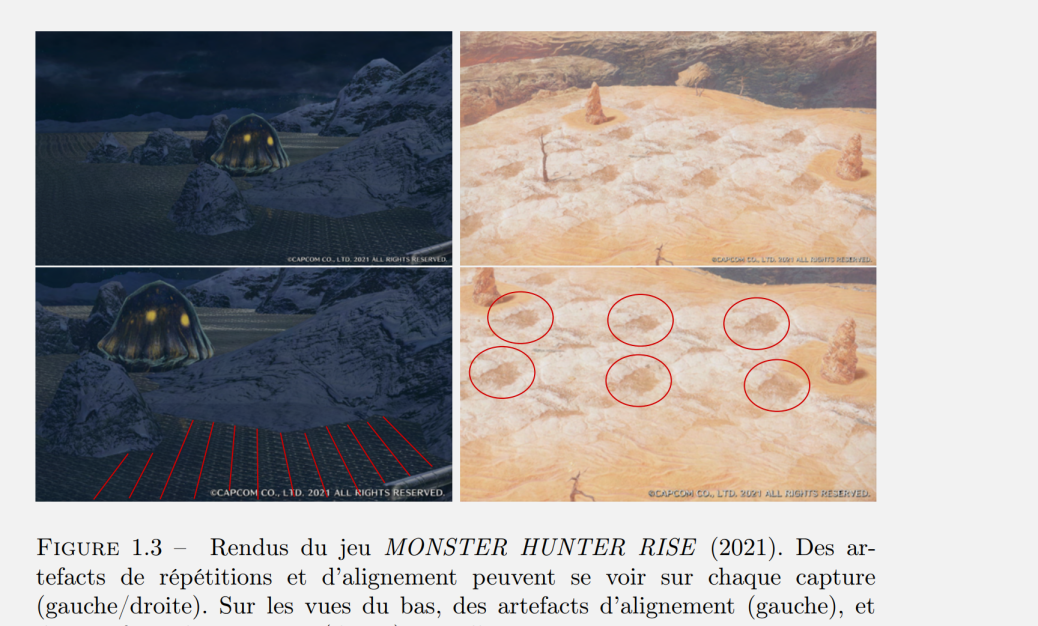
\includegraphics[width=\textwidth]{contenu/resources/images/periodic_tiling}
    \caption[Artefacts d'alignement créés par le pavage périodique]{Artefacts d'alignement créés par le pavage périodique, \textit{Monster Hunter Rise} (2021), Capcom. Crédits à N. Lutz~\cite{lutz_processus_2021} pour l'image}
    \label{fig:pavage_periodique}
\end{figure}

On préfère en général prendre des tuiles plus petites et mieux les mélanger~\cite{heitz_high-performance_2018} afin de d'obtenir de la variété et d'éviter la répétition de motifs saillants.
% TODO "motifs saillants" dualité cohérence vs variété, importance de la taille de la tuile (G)
% TODO def variété + motifs saillants, pourquoi on veut variété, pourquoi on veut pas répét motifs saillants


\subsubsection{Synthèse par convolution}

% TODO def noyaux
L'objectif d'une synthèse par convolution est de construire une texture en disposant des motifs, appelés \og noyaux \fg, selon une distribution statistique. Le choix du noyau, de la distribution, ainsi que de la méthode de mélange, sont les paramètres à ajuster pour contrôler la synthèse. Une pratique habituelle de la synthèse par convolution est de choisir comme noyau une somme d'ondelettes (typiquement des cosinus) spatialement contraintes et à orientation aléatoire, et de contrôler les fréquences des ondelettes utilisées~\cite{tricard_procedural_2019}. En sélectionnant les fréquences, on a un contrôle sur le contenu fréquentiel présent dans la texture produite, ce qui permet une bonne maîtrise de l'apparence générée~\cite{gilet_local_2014}.

\bigskip

% DIRE QUE LA SYNTHESE DE MOTIFS OU DE STRUCTURE EST ENCORE TRES COMPLIQUEE
Les méthodes existantes de synthèse ne fonctionnent cependant pas bien lorsque la cible contient des motifs organisés ou de la répétition. Quelques tentatives ont été faites~\cite{lutz_cyclostationary-gaussian_2021} pour synthétiser des textures présentant une forme de structure et régularité, mais en dehors de configurations présentant des caractéristiques particulières, comme une certaine périodicité, la synthèse de structure irrégulière est compliquée.
% TODO image pour appuyer dernière ligne + mieux expliquer pourquoi
% TODO contribution \cite à décrire. Tu peux aussi citer l'article sur la préservation de l'autocovariance

% \section{Génération procédurale} % Non-nécessaire ? De quoi on parle ici sinon ?

% \section{Bruit procédural}

\section{Analyse multi-résolutionnelle locale}

Une des raisons pour lesquelles la synthèse de texture contenant de la structure est difficile est qu'il faut préserver certaines relations entre les texels de l'image pour garder la structure. Savoir quelles relations préserver, pour garder la structure de l'image, et quelles relations supprimer, pour ajouter de la variation dans la synthèse, est très délicat, surtout dans le contexte du temps-réel. L'idée explorée dans cette recherche est d'appliquer des outils de l'analyse d'image, outils capables d'extraire des caractéristiques d'une image par l'analyse de relations intra-image, à des processus de synthèse.
% TODO question à soulever plutôt qu'affirmation à faire
% qu'est ce qu'une structure ? mieux introduire avec la partie d'après
% TODO Suggestion : parler de "relations statistiques" plutôt que de "relations", et dire qu'il faut les préserver au mieux. Tu veux préserver toutes les relations statistiques, mais certaines sont trop complexes à préserver en temps réel, en plus d'être difficiles à "capturer". C'est pour ça que tu essayes de développer les outils suivants.
% TODO très délicat = trop vague

\subsection*{Notion de structure}

La structure d'une image désigne comment les différentes parties de l'image sont agencées les unes par rapport aux autres, comment les éléments de l'image forment certains schémas ou présentent une certaine forme de régularité. Ces relations sont présentes à différents niveaux d'échelle, on a donc différents niveaux de structure. Savoir quels niveaux préserver et comment est important pour reproduire les caractéristiques désirées de la texture.

\begin{figure}[h!]
    \centering
    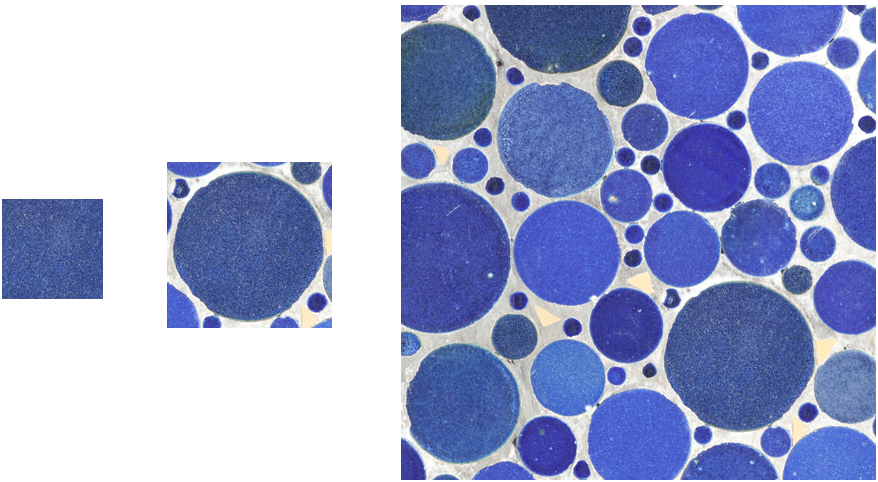
\includegraphics[width=.85\linewidth]{contenu/resources/images/structure_level}
    \caption{Différents niveaux de structure au sein d'une image}
    \label{fig:structure_level}
\end{figure}

\subsection*{Congruence de phases}

Lorsque l'on veut préserver la structure d'une image, les éléments saillants tels que des coins et des lignes, ou plus généralement des bords, sont compliqués à reproduire. On appelle \og bord \fg une région frontière entre un objet et un autre élément de l'image, comme l'arrière plan ou un autre objet. Visuellement, un bord se distingue par un changement brusque de luminosité. Ces changements sont cependant plus difficiles à détecter automatiquement, car le seuil minimum de contraste entre des pixels voisins n'est pas toujours le même, dépendamment de si le bord est franc ou flou. Une approche intéressante est d'utiliser des informations du domaine fréquentiel pour caractériser des bords.
% TODO /!\ luminosité terme nouveau à mieux definir
% p-e image pour illustrer
% TODO "compliqué à reproduire" pourquoi ?
% TODO source pour utilisation domaine fréquentiel

\bigskip

Lorsqu'une image est décomposée dans le domaine de Fourier, on retrouve de nombreuses informations sur la structure dans la phase~\cite{oppenheim_importance_1981}. En explorant le rôle de la phase, Kovesi a mis au point un outil de détection de d'éléments caractéristiques~\cite{kovesi_image_1995} basé sur le modèle physiologiquement réaliste d'énergie locale de Morrone et al.~\cite{morrone_feature_1987, morrone_feature_1988}. Ce modèle postule que les éléments caractéristiques sont présents dans une image là où les composants de Fourier sont maximalement en phase. La congruence de phases qui dérive du modèle d'énergie locale est une grandeur qui quantifie cet alignement. Elle donne lieu à un outil de détection plus robuste que ceux développés auparavant, qui sont souvent sensibles au niveau d'illumination et de grossissement, et nécessitent donc une connaissance a priori des images étudiées. C'est ce modèle de congruence de phases que nous avons repris et adapté à la synthèse de texture.
% TODO paragraphe trop rapide
% étendre et reposer la problématique
% notamment vis a vis de l'aléatoire, préserver congruence avec aléatoire est le noeud du pbl
% todo introduire PC avant de juste en parler

\bigskip

\begin{figure}[h]
    \centering
    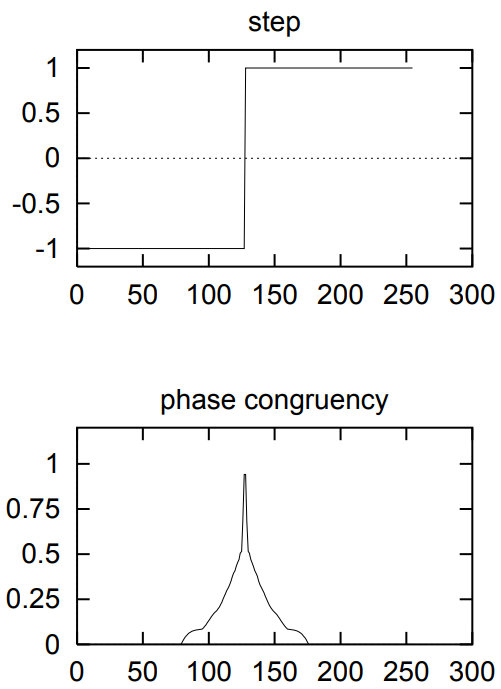
\includegraphics[width=.35\linewidth]{contenu/resources/images/pc_1d_kovesi}
    \caption[Congruence de phases pour un signal 1D]{Congruence de phases pour un signal 1D, Kovesi (1995)~\cite{kovesi_image_1995}}
    \label{fig:pc_1d_kovesi}
\end{figure}

Pour détecter un alignement de phase, il est nécessaire d'avoir un modèle donnant des informations locales sur notre image. Kovesi utilise pour cela une banque de filtres à orientation variable. Nous utilisons à la place le modèle mathématique de la transformée de Riesz, qui permet de décomposer une image dans un espace différent, similairement à la transformée de Fourier, mais avec des informations locales, au niveau du texel (on rappelle que la transformation de Fourier fournit des informations fréquentiellement locales, mais spatialement globales). Utiliser cette transformée nous permet ainsi d'étudier la présence et préservation de relations dans un autre espace que le domaine spatial, donc de mieux comprendre et caractériser nos images.
% TODO dernière ligne : comment pourquoi dans quel but pour atteindre quoi ?

\subsection*{Analyse multi-échelle}

% TODO première phrase : pourquoi ? répond a quel besoin ?
Un objectif de la méthode présentée ici est de pouvoir agir avec précision sur certains niveaux d'échelle de structure ciblés. Une méthode d'analyse qui permet de travailler avec plusieurs niveaux de résolution de la même image est dite \og multi-résolutionnelle \fg~\cite{mallat_theory_1989}, ou multi-échelle. Des exemples d'application communs de méthodes d'analyse multi-résolutionnelle sont la détection robuste de caractéristiques de différentes tailles~\cite{park_multiresolution_2010} et la compression d'images~\cite{averbuch_image_1996}.
%TODO étendre et mieux expliquer. intégrer la phrase d'après qui a été coupée du texte
On décompose notre image en pyramide d'images, ce qui nous permet d'étudier les différences de détails entre les différents niveaux d'échelle.

\section{Plan du manuscript} % / problématique

Ce manuscrit est organisé comme suit :

\begin{itemize}
%    \item revue de l'état de l'art de la synthèse de texture temps réel,
    \item explication de la théorie de Riesz et du modèle d'analyse multi-échelle local qui en découle,
    \item application à la synthèse de texture par échantillonnage préférentiel.
\end{itemize}